\subsection{RDF Vocabulary}

The need for a decentralized mechanism for publishing information whose 
\emph{meaning} is machine-readable has been known for more than two decades
\textcolor{red}{cite https://www.w3.org/Talks/WWW94Tim/}. Since then a 
collection of tools and technologies - the Semantic Web - has accumulated, with
perhaps the most significant being the specification of RDF as a data 
interchange format for the World Wide Web. \textcolor{red}{cite https://www.w3.org/RDF/?}
In RDF \emph{things} (concepts or concrete items) are represented as URIs
and arranged in \emph{triples} of a subject, a predicate and an object. 

\begin{figure*}
\begin{minted}{turtle}
@prefix nersc: <http://portal.nersc.gov/project/mpccc/sleak/nersc#> .
@prefix rdfs: <http://www.w3.org/2000/01/rdf-schema#> .
@prefix foaf: <http://xmlns.com/foaf/0.1/> .
nersc:nersc rdfs:type foaf:Organization .
\end{minted}

\caption{A triple of (subject, predicate, object) describes an edge 
in an RDF graph. The \texttt{Turtle}\textcolor{red}{cite} syntax shown
here aids human readability by condensing URIs into a prefix and a suffix,
so for example \texttt{rdfs:type} expands as
\texttt{<http://www.w3.org/2000/01/rdf-schema\#type>}.}
\label{f:rdftriples}
\end{figure*}

For example, we wish to state that NERSC is an Organization. We have a 
\emph{subject} (NERSC), a \emph{predicate} (``is an'') and an \emph{object} 
(Organization). In a manner of pulling oneself up by one's bootstraps, the 
W3C \textcolor{red}{cite https://www.w3.org/} publishes some standard 
vocabularies in the form of URIs that have a well-defined and documented 
meaning, including that \texttt{<http://www.w3.org/2000/01/rdf-schema\#type>}
refers to the predicate ``is a''. Another vocabulary, known as the 
Friend-of-a-friend vocabularies, associates \texttt{<http://xmlns.com/foaf/0.1/Organization>} with the concept of an 
organization. In this spirit we write the triple in Figure~\ref{f:rdftriples}
by associating the 
we've chosen to associate the URI \texttt{<http://portal.nersc.gov/project/mpccc/sleak/nersc\#nersc>} with the 
organization we know as ``NERSC''. 

Notice that our URI doesn't actually say anything \emph{about} NERSC, not even 
that it is called ``NERSC''. In reality, it is simply a URI within a 
namespace we control. But we can add more triples to the graph such as
that our chosen URI has a ``name'' (using another pre-defined predicate)
with the literal value ``NERSC''. Moreover, we can publish a document 
at \texttt{<http://portal.nersc.gov/project/mpccc/sleak/nersc>} containing 
these and other triples. Now the URI we chose for NERSC corresponds to an 
anchor within this document, so an application that encounters a reference 
to this URI can fetch that document and infer more about NERSC.

% this is a key point
\begin{keypoint}
A collection of triples forms a graph whose edges have well-defined meanings, 
allowing information about nodes to be inferred from their relationships to 
other nodes.
\end{keypoint}

Note that in the example we defined prefixes and used a shorthand form of 
the URIs. A variety of syntaxes exist to describe RDF in a more human-readable
manner, so for the remainder of this article we will use this \texttt{Turtle}
syntax. 

By using web-based URIs as identifiers we get a mechanism for a distributed,
decentralized graph of knowledge. An application encountering a URI can 
choose to simply accept it as a unique identifier, or to incorporate its
namespace into the application's knowledge graph.

Crucially, an RDF graph can be queried using SPARQL \textcolor{red}{cite}, a
graph-query language with a look-and-feel similar to SQL. A SPARQL query 
arranges variables into a set of triples and returns nodes for which
the triples form a true statement. For example, the following SPARQL query
will return the name and interest for each node whose type is 
a subclass of \texttt{foaf:Agent}. \texttt{foaf:Agent} is a superclass for a Person, a 
Group or an Organization, so this query in English is ``list the name and 
interest for each Person, Group or Organization in this graph''. (The 
\texttt{rdfs:subClassOf*} syntax indicates that the query should follow 
\texttt{rdfs:subClassOf} edges to any depth until a \texttt{foaf:Agent} 
is encountered).

Figure~\ref{f:sparql-diagram} illustrates how this query might act on a graph: 
the first statement locates nodes from which one can traverse \texttt{rdfs:subClassOf} properties and reach a \texttt{foaf:Agent} - colored blue. The second statement 
locates nodes in triples with an \texttt{rdfs:type} predicate whose object 
is one found by the first statement - shown here in red. Thus far we have found Jim, 
Ann, Annette and Steve. Next we look for triples whose subject is one of those nodes
and whose predicate is \texttt{foaf:name}, reducing the set to Jim, Ann and Steve, then
again for predicate \texttt{foaf:interest}. Now only Steve matches all of the criteria.
Finally, we return the nodes associated with the \texttt{name} and \texttt{interest} 
variables, which in this case are the purple-colored objects of those triples.


\begin{figure}[H]
\begin{minted}{sparql}
SELECT ?name ?interest 
WHERE {    
    ?type rdfs:subClassOf* foaf:Agent .
    ?uri rdfs:type ?type .
    ?uri foaf:name ?name .
    ?uri foaf:interest ?interest .
}
\end{minted}
\caption{Example of a SPARQL query}
\label{f:sparql}
\end{figure}


\begin{figure*}
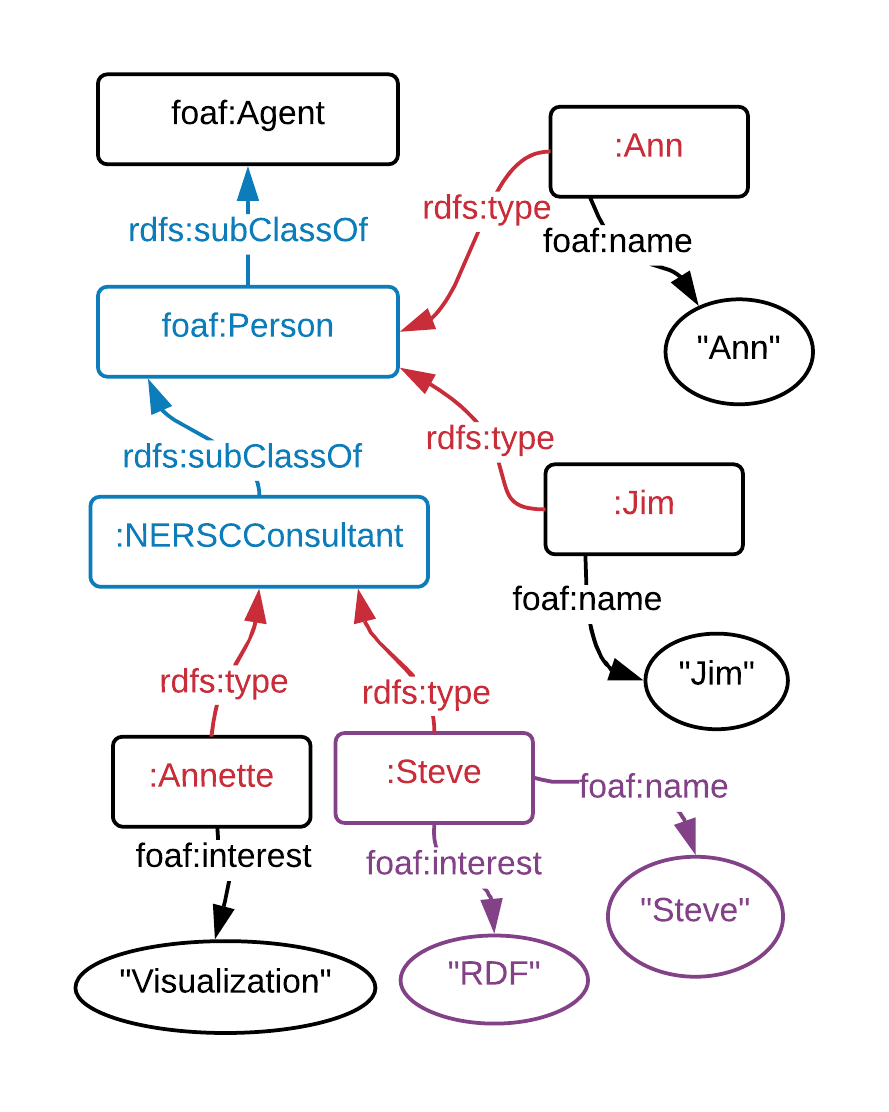
\includegraphics[width=0.9\textwidth]{sparql.png}
\caption{Illustration of the SPARQL query in Figure~\ref{f:sparql} }
\label{f:sparql-diagram}
\end{figure*}

\textcolor{red}{TODO: draw this as a diagram, probably explains it better}
\textcolor{red}{TODO: prob need a ref to an "intro to semantic web" resource}

RDF provides a decentralized mechanism for publishing information in a
machine-readable and searchable way, neatly meeting our requirements
(2) and (5). Furthermore, RDF allows us to use an established ecosystem of 
tools and libraries to achieve our goals.

\subsubsection{The vocabulary}

The key classes and predicates forming our vocabulary are illustrated in Figure~\ref{f:logset-classes}. The vocabulary is extended and specialized from the Data Catalog Vocabulary \textcolor{red}{cite}. The meaning, reason and usage of each are as follows:

\begin{description}
\item[Catalog] 
The \texttt{dcat:Catalog} class is used as an access point to LogSet datasets and 
to link disparate collections into a single graph. Catalogs are anticipated to be 
published at a site granularity: staff at a site would publish the LogSets 
at whatever URL each individual can access 
\item[LogSet] 
A collection of logs related in system and access and timespan,
for example the logs collected in a \texttt{p0-} directory in the SMW of a Cray
XC for a single boot session. A LogSet might be made available would normally be made available 

\end{description}


\textcolor{red}{TODO include a diagram}


-- some key things to call out:
\begin{itemize}
\item someone publishing a logset doesn't need to know many people to get their 
      logset into the graph - a curator of their local (site) catalog is enough. 
      That curator then knows curators of at least one other catalog and thus 
      gets the local 
      subgraph into the global graph
\item someone using the graph doesn't need to know who published what - they can
      query the graph itself and get metadata about what is out there, including contact 
      information for data they don't directly have access to. This allows them to 
      solve specific access limitations in a locally-appropriate way
\end{itemize}

\begin{figure*}
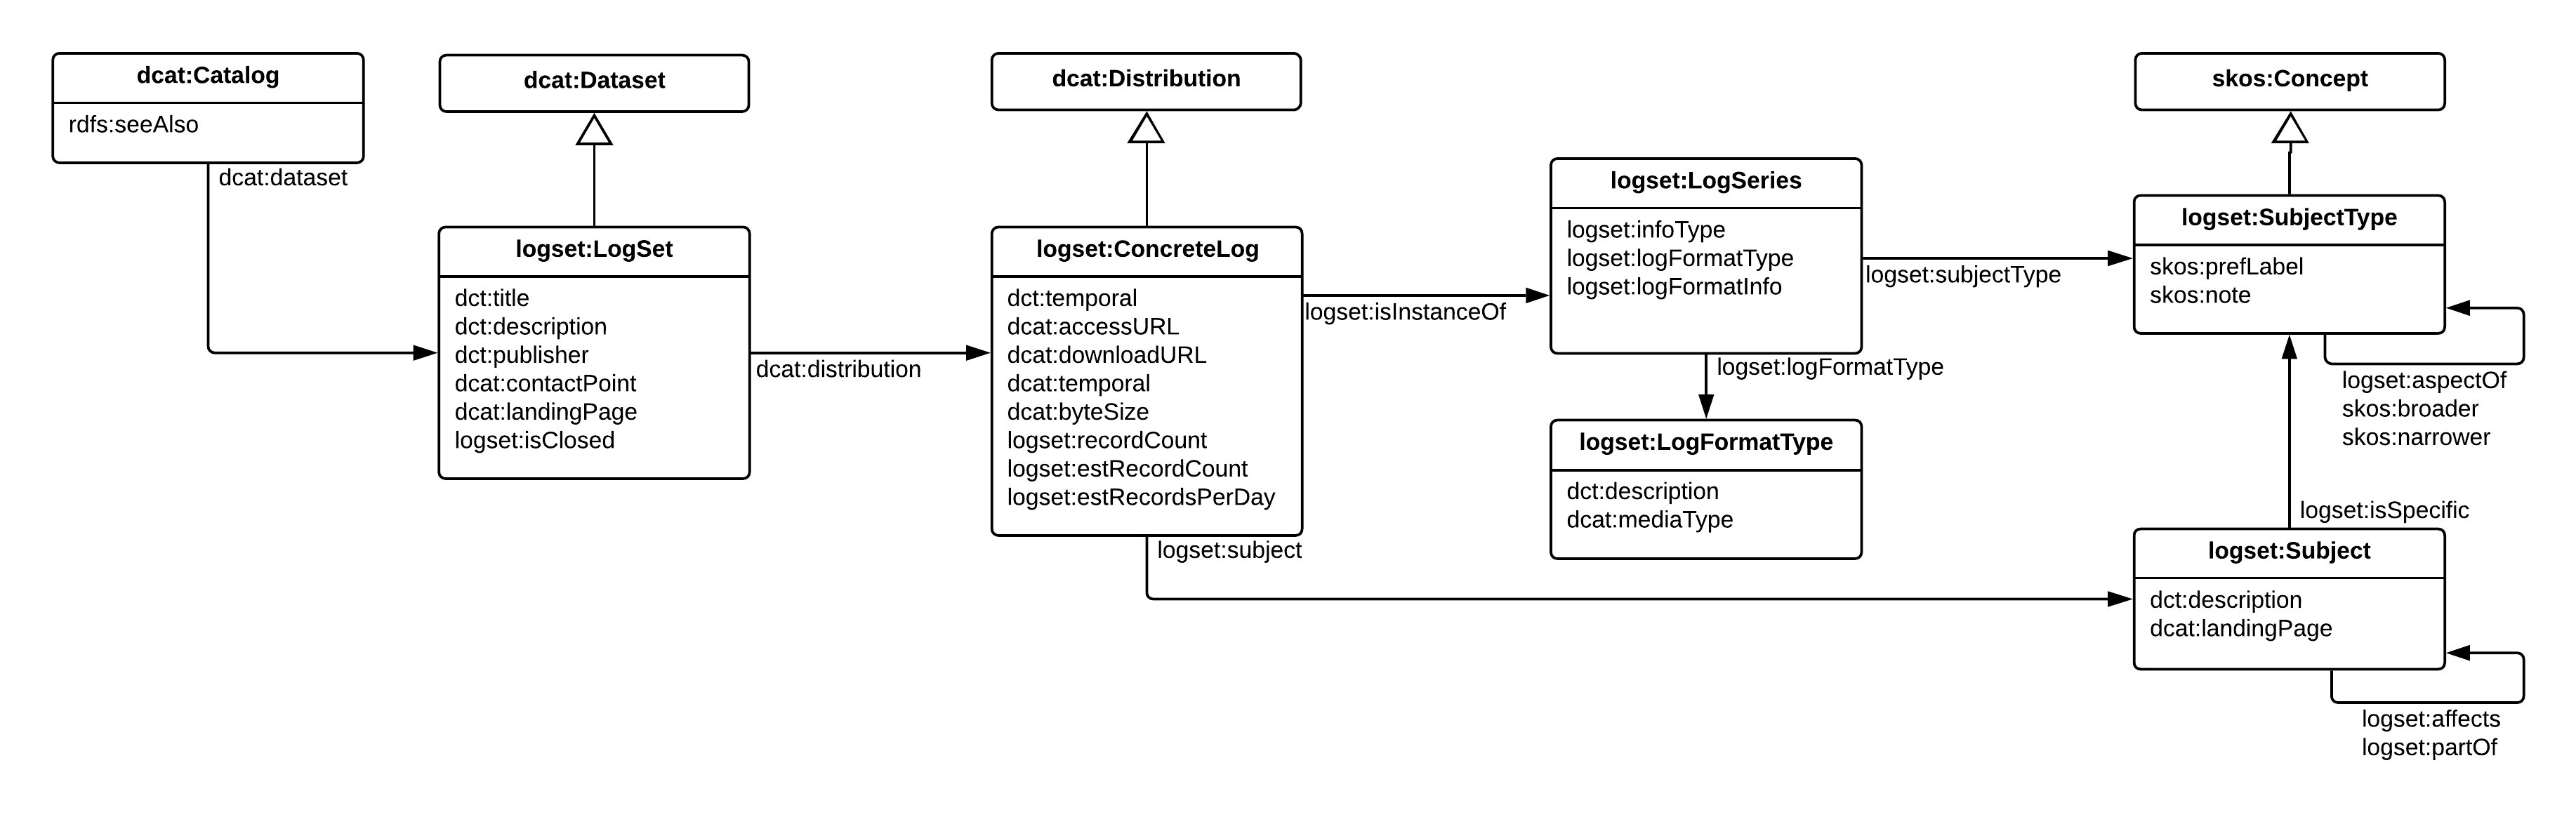
\includegraphics[width=0.9\textwidth]{logset-key-classes.png}
\caption{Key classes and predicates in the logset vocabulary. }
\label{f:logset-classes}
\end{figure*}

